\documentclass{article}
\usepackage[T1]{fontenc}
\usepackage{lmodern}
\usepackage{graphicx}
\usepackage{amsmath,amssymb}
\usepackage[a4paper,margin=2cm]{geometry}
\usepackage[absolute,overlay]{textpos}
\setlength{\TPHorizModule}{1mm}
\setlength{\TPVertModule}{1mm}
\usepackage[indonesian]{babel}
\usepackage{hyperref}
\setlength{\emergencystretch}{2em}
% unit: Halaman 17

\begin{document}

% === Halaman 17 (llm) ===

\vspace{129.79mm}

Metode Enhanced LSB

% deskripsi: Ilustrasi proses modifikasi bit LSB (Least Significant Bit) pada komponen warna Blue, Green, dan Red, menunjukkan perubahan nilai biner dari warna asli menjadi nilai maksimal atau minimal.
% bbox normalisasi: [0.1580, 0.2740, 0.8370, 0.3980]
\begin{textblock*}{142.59mm}(33.18mm,81.38mm)
\noindent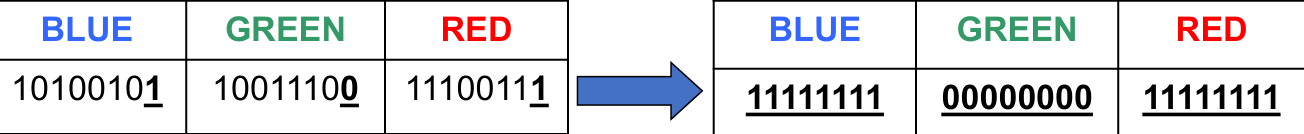
\includegraphics[width=142.59mm,height=36.83mm]{../../images/llm/page_017_img_01.png}%
\end{textblock*}

% deskripsi: Perbandingan gambar kincir angin sebelum (kiri) dan sesudah (kanan) diterapkan metode Enhanced LSB, di mana gambar kanan menunjukkan noise warna yang signifikan.
% bbox normalisasi: [0.1930, 0.4750, 0.7780, 0.9120]
\begin{textblock*}{122.85mm}(40.53mm,141.07mm)
\noindent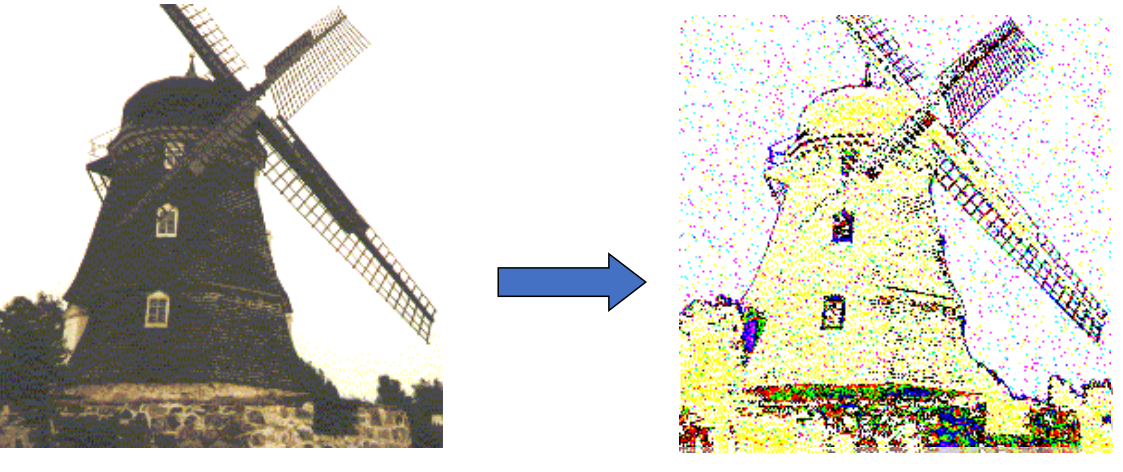
\includegraphics[width=122.85mm,height=129.79mm]{../../images/llm/page_017_img_02.png}%
\end{textblock*}

\end{document}
